\section{Block Time}

\subsection{Proof-of-Work}
\label{diff_adjustment}

In Ethereum's PoW system, the block time — the average time
interval between blocks — is primarily governed by a difficulty adjustment
algorithm. This algorithm dynamically alters the computational difficulty of
mining a block, striving to keep the block time within a targeted range.
The algorithm was implemented in the Ethereum Improvement Proposal 2 (EIP-2),
it adjusts difficulty levels based on observed block times \cite{eip-2}:

\begin{itemize}
  \item If the block time falls short of the ideal duration (less
    than 10 seconds), the difficulty is increased. This escalation in
    difficulty slows down the rate at which new blocks are mined,
    counteracting the tendency towards overly rapid block generation.

  \item Conversely, if the block time stretches beyond the desired limit (exceeding
    20 seconds), the difficulty is decreased. This reduction makes it easier to
    mine new blocks, compensating for excessively lengthy block intervals.
\end{itemize}


The follwing pie chart offers a visual representation of Ethereum's block time
distribution under PoW throughout 2021. As anticipated, the block times
exhibited considerable variability, averaging around 13.4 seconds


\begin{figure}[H]
  \centering
  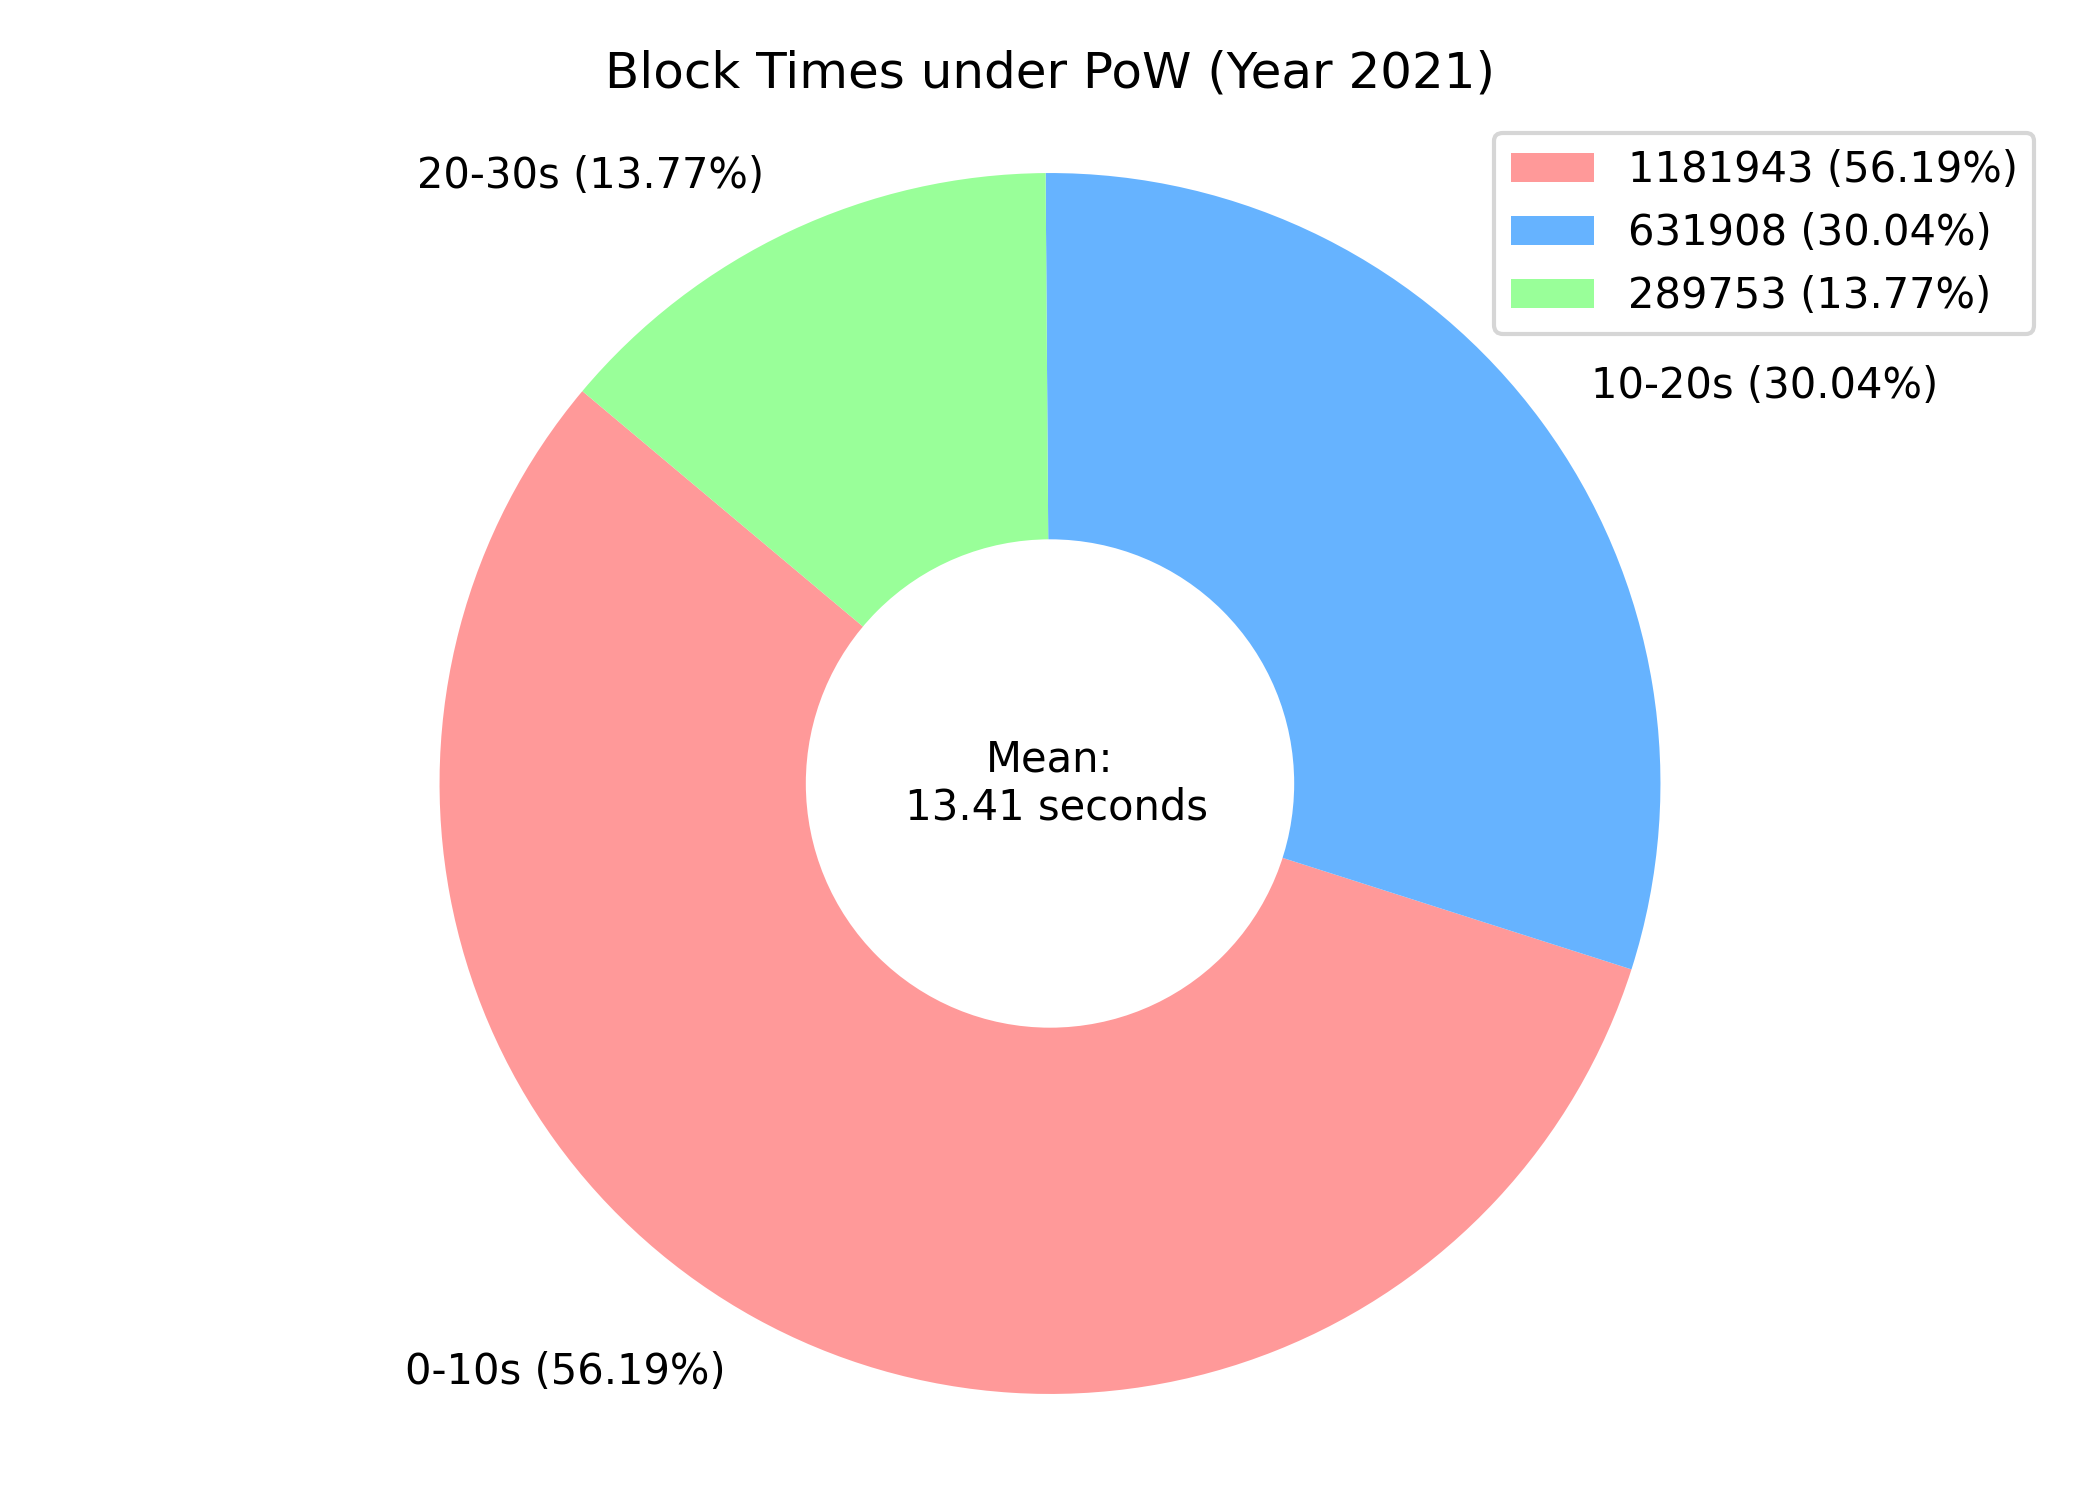
\includegraphics[width=0.8\textwidth]{block_time_analysis/pow_block_time_pie_chart.png}
  \caption{Block times under PoW in the year 2021.}
  \label{fig:block_time_analysis_pow}
\end{figure}

\subsection{Proof-of-Stake}
\label{pos_block_time}
%Following 'The Merge' on September 15, 2022, Ethereum has shifted to a
%PoS consensus mechanism \cite{eth_history}. Under PoS, validators propose new
%blocks, with a selection process involving other validators who vote to confirm
%these blocks authenticity. A stake of 32 ETH is required to be locked in as a
%deposit for one to become a validator. This staking mechanism ensures validator
%honesty, as any malpractice could lead to the loss of their staked ETH.

The newly adopted PoS system is organized around slots and epochs, with slots
being 12-second
intervals and an epoch consisting of 32 such slots
\cite{seconds-per-slot-mainnet}\cite{seconds-per-slot-mainnet-doc}. For each
slot a validator is chosen by the protocol's algorithm to propose a new block.
In the event that the selected validator, responsible for proposing a new
block, is offline, the slot remains empty
\cite{validator-offline}.

Each block within a slot corresponds to the slot's specific timestamp.
Consequently, the typical interval between blocks is approximately 12 seconds.
However, there are exceptions: if a slot remains unoccupied, the time interval
for the subsequent block extends to 24 seconds, and this pattern continues
accordingly (36,48,..).

An examination of the blockchain data since the Merge \footnote{starting at block number
15537393} reveals that 99.05\% of all blocks have been consistent with a block
time of 12 seconds, as shown in Figure
\ref{fig:block_time_analysis}.

\begin{figure}[H]
  \centering
  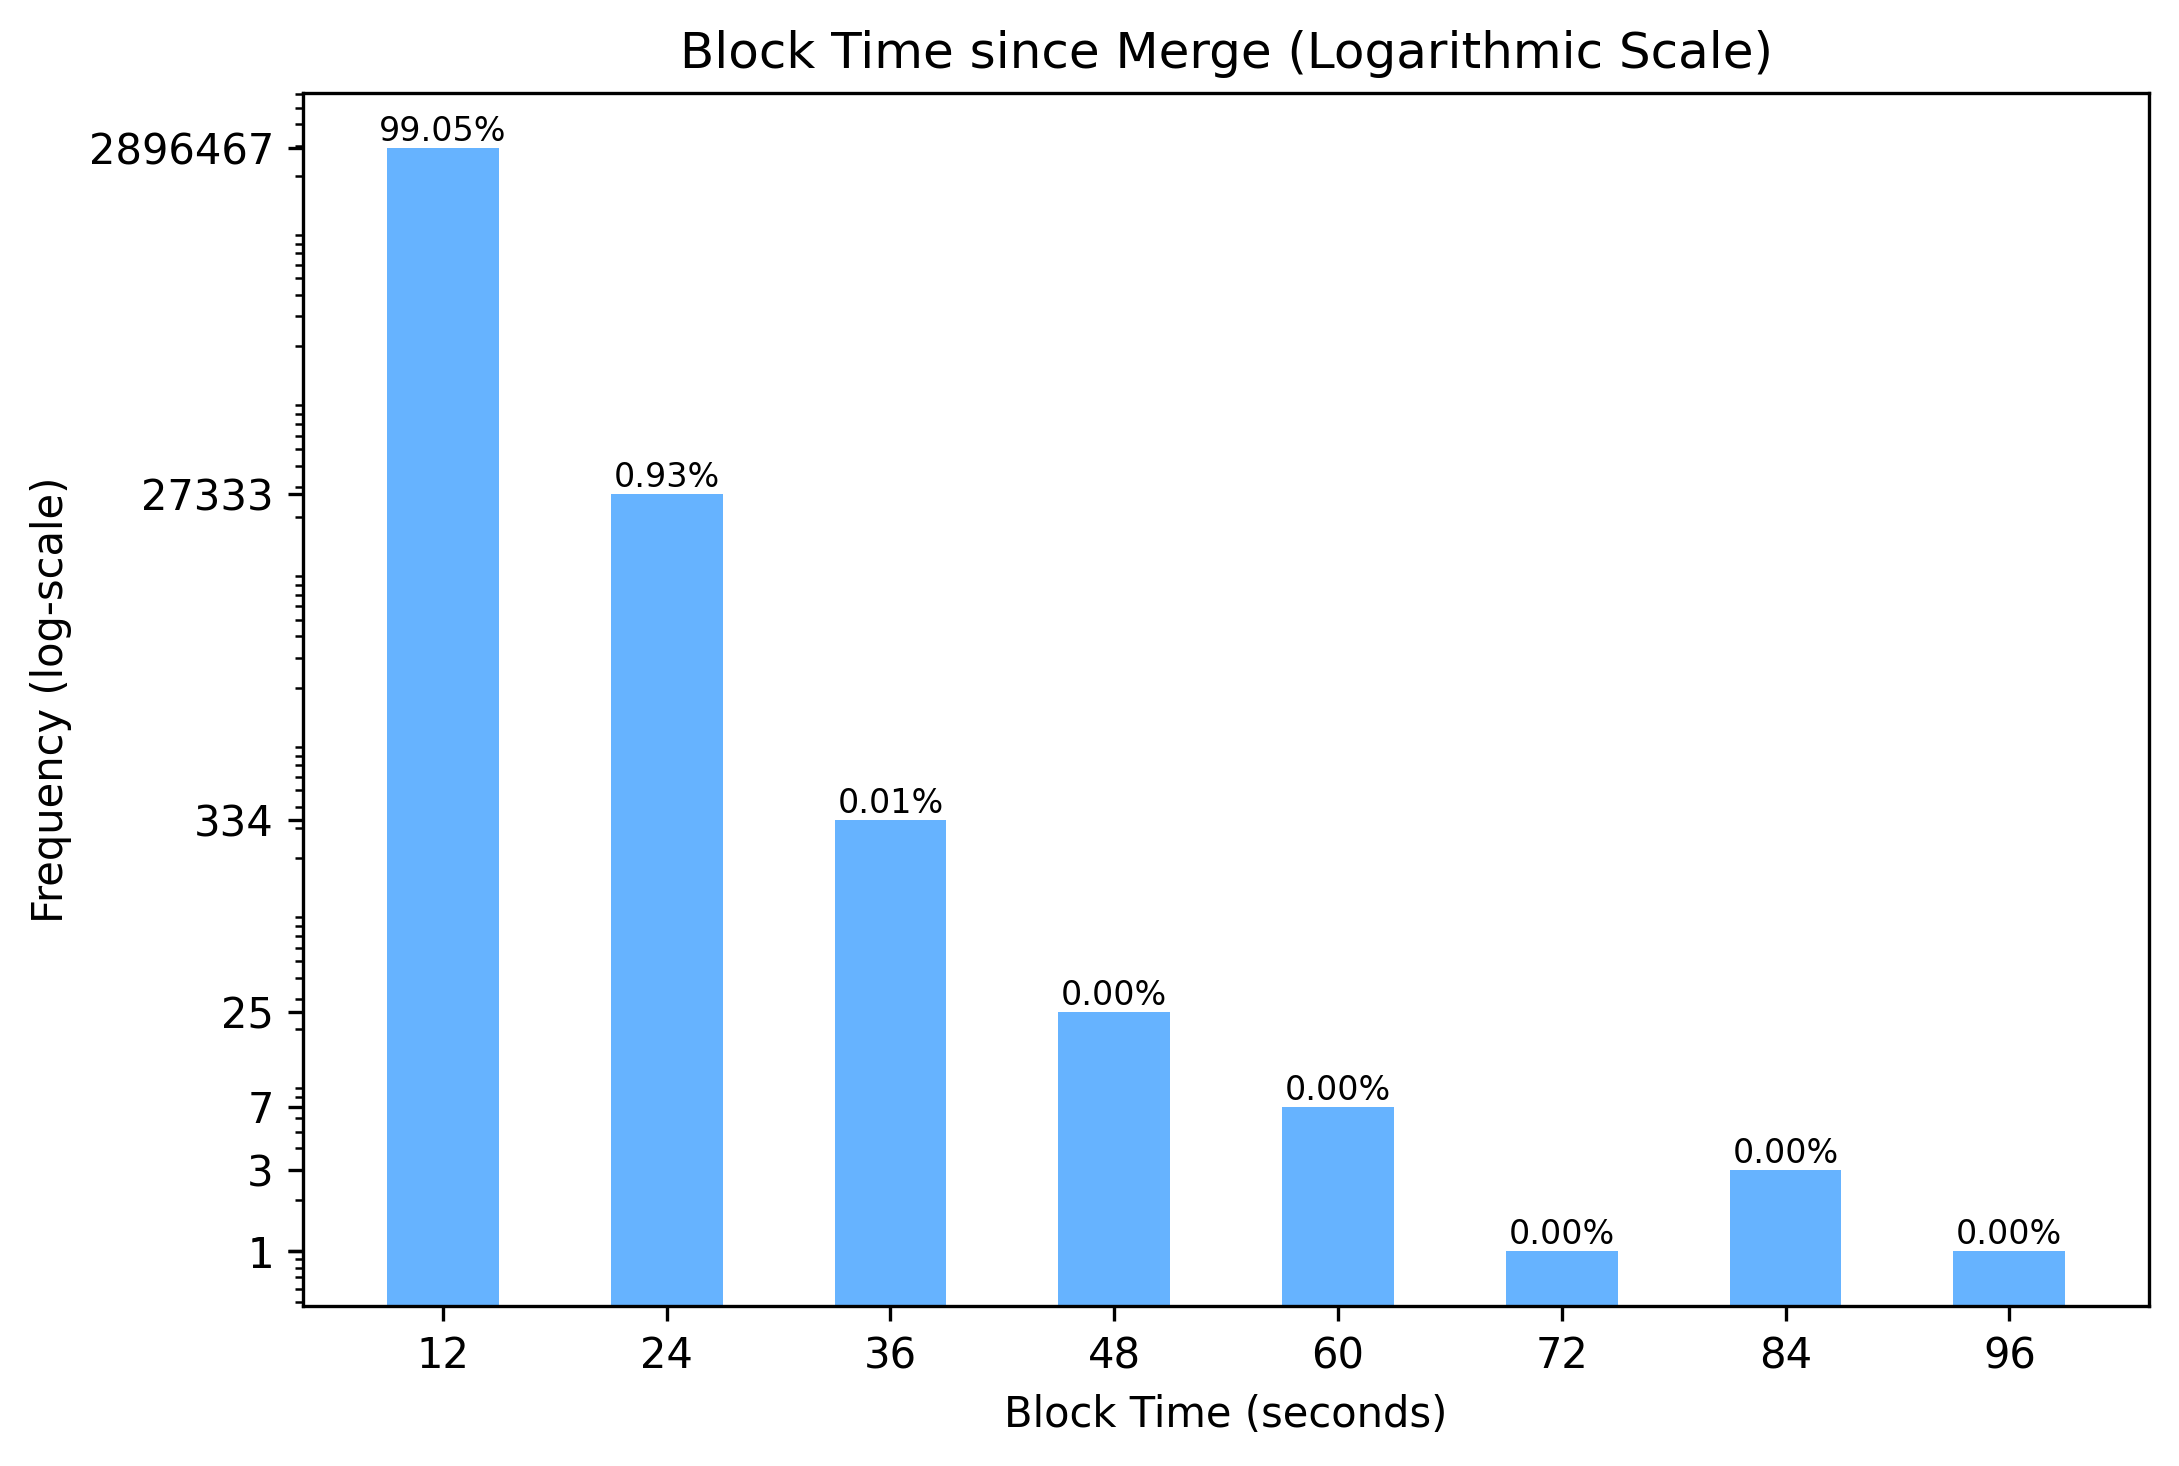
\includegraphics[width=1\textwidth]{block_time_analysis/pos_block_time_bar_chart_with_percentages.png}
  \caption{Block times since the merge (block numbers: 15537394 to 18461556).}
  \label{fig:block_time_analysis}
\end{figure}

